\chapter{Einführung}
\vspace{-2cm}
\label{chap:Einführung}
In diesem Kapitel werden die theoretischen Grundlagen der Antennen-und Leitertheorie gelegt sowie das SatNOGS Netzwerk näher erläutert.
\vspace{-2cm}
\section{SatNOGS-Netzwerk}
\label{sec:sat}
Das SatNOGS-Netzwerk spielt eine zentrale Rolle in unserer Diplomarbeit und bietet hunderten Forschern, Amateurfunkern und Interessierten eine Plattform für verlässliche Kommunikation mit Satelliten.\\
\newline
Das, was SatNOGS zu so einer attraktiven Lösung macht, ist der Fakt dass die Bodenstation um den ganzen Globus verteilt sind. Der große Vorteil davon ist, dass der Empfang von Satellitendaten nun über alle verfügbaren Empfangsstationen laufen kann.\\
\newline
In Abbildung \ref{fig:SatNOGS_Erklärung} wird die Topologie des SatNOGS-Netzwerkes abstrahiert dargestellt.
Alle über das Netzwerk verfügbaren Bodenstationen sind mit SatNOGS-Servern verbunden. Auf diese Server kann über die Website bzw. API zugegriffen werden, welche die empfangenen Satellitendaten für alle Benutzer erreichbar macht.

\begin{figure}[H]
	\centering
	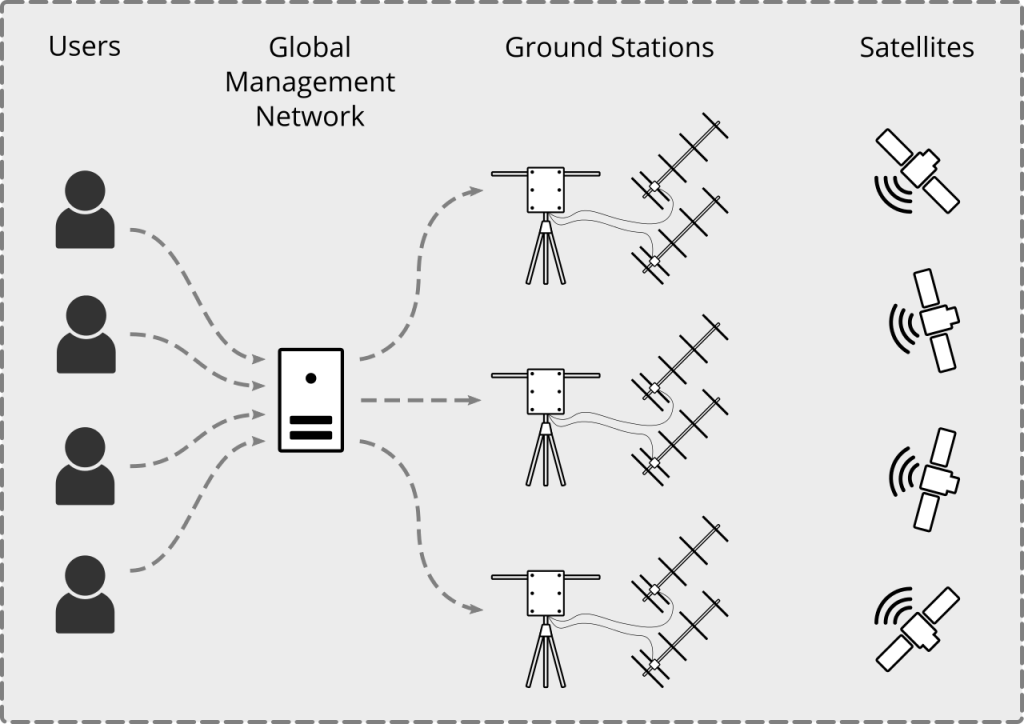
\includegraphics[width=\textwidth]{../ref/SatNOGS_explanation}
	\caption{Erklärung des SatNOGS Netzwerkes}
	\label{fig:SatNOGS_Erklärung}
\end{figure}	

\begin{figure}[H]
	\centering
	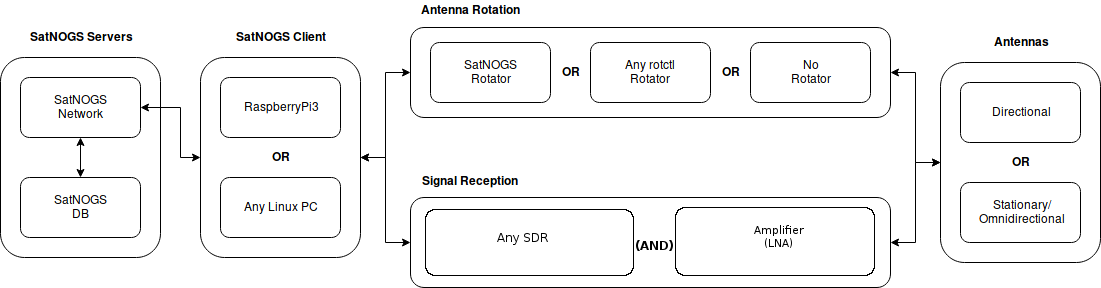
\includegraphics[width=\textwidth]{../ref/SatNOGS_BlockDiagram}
	\caption{SatNOGS-Systemtopologie}
	\label{fig:SatNOGS_Systemtopologie}
\end{figure}

Um näher auf den Ablauf des Datenempfangs und der benötigten Systemblöcke einzugehen wird auf Abbildung \ref{fig:SatNOGS_Systemtopologie} verwiesen.\\
\newline
Zum Empfang von Daten kommen zwei Antennentypen infrage: Direktionale oder omnidirektionale Antennen. Eine direktionale Antenne folgt dem Verlauf des Satelliten. Dies bringt den Vorteil mit sich, dass eine höhere Empfangsleistung erzielt, und somit klarere Daten empfangen werden, jedoch wird für solch ein Modell ein Rotator benötigt. Der Vorteil einer omnidirektionalen Antenne ist, dass kein teurer Rotator notwendig ist, allerdings können damit nur schwer brauchbare Daten empfangen werden.\\
\newline
Für gerichtete Antennen können verschiedene Rotatoren benutzt werden, unter anderem der "SatNOGS-Rotator" sowie diverse Open-Source-Rotatoren und Rotatoren welche zum Verkauf stehen.\\
\newline
Zur Demodulation der Daten sind ein SDR (Software Defined Radio) sowie ein LNA (Low Noise Amplifier) notwendig. Das SDR übernimmt softwaretechnisch Aufgaben welche normalerweise von Hardware übernommen werden (Demodulation, Filter, Mixer, etc...). Der LNA, wie der Name schon andeutet, ist für die Verstärkung kleiner Signale mit besonderer Rauscharmut verantwortlich. \\
\newline
Die Aufgabe des SatNOGS Clients kann in der Regel von jedem Linux-PC oder RaspberryPi übernommen werden. Allerdings wird die Kompatibilität zwar für alle Linux-basierten PCs, jedoch nur für die RaspBerryPis Version 3, 3+ und 4 garantiert.\\
\newline
Der SatNOGS Client ist mit den Servern verbunden, der die Bodentation als solche im Netzwerk repräsentiert. Die Server unterhalten weiters eine Datenbank, welche Daten über Satelliten enthält, die mit den Empfangsstationen erreichbar sind.
\pagebreak

\section{grundlegende Antennentheorie}
\label{sec:basic-ant}
\subsection{Einführung}
Um die in der Diplomarbeit bearbeiteten Inhalte besser verstehen zu können, wird eine Einführung in die Grundlagen der Antennentheorie gegeben. 

\subsection{Antennenfeldzonen}
Das von einer Antenne abgestrahlte Feld lässt sich in 3 verschiedene Regionen einteilen: das Nahfeld, das Übergangsfeld (Fresnel-Region) und das Fernfeld (Fraunhofer-Region).\\
\newline
Je nach Literatur erfolgt der Übergang zwischen den Feldzonen fließend. Eine Möglichkeit die Zonen einzuteilen ist in der nachfolgenden Tabelle einzusehen.

\begin{center}
	\begin{tabular}[h]{|c|c|c| p{"5"cm}}
		\hline
		Nahfeld & Übergangsfeld & Fernfeld\\
		\hline
		r $<$ 0.2 $\lambda$ & 0.2 $\leq$ r $\leq$ 4$\lambda$ & r $>$ 0.4$\lambda$\\
		\hline
	\end{tabular}
\end{center}

Das Nahfeld ist darin besonders, dass das elektrische und magnetische Feld mit unterschiedlichen Faktoren in Abhängigkeit der Entfernung abnehmen. Im Übergangsfeld nehmen das elektrische und magnetische Feld zwar mit dem gleichen Faktor ab, jedoch unterscheiden Sie sich noch in der Phase und Amplitude.\\
\newline
Im Gegensatz zum reaktiven Nahfeld wird beim Fernfeld Wirkleistung abgestrahlt. Hierbei sind die elektrische und magnetische Komponente der Welle in Phase und nehmen im gleichen Maß ab.\\
\newline
Da unsere Diplomarbeit einen Fokus auf die Satellitentechnik hat, ist für dieses Dokument nur das Fernfeld relevant. 

\subsection{Polarisation}
Die Polarisationsart wird von der Ausrichtung des Vektors der elektrischen Feldstärke bestimmt. Es lässt sich zwischen drei verschiedenen Arten der Polarisation unterscheiden.\\
\newline

\begin{itemize}
	\item Lineare Polarisation
	\begin{itemize}
		\item horizontale Polarisation\\
		Eine horizontale Polarisation liegt vor, wenn der elektrische Feldstärkevektor sich periodisch ändert und die Feldlinien parallel zum Boden verlaufen.
		\item vertikale Polarisation\\
		Eine vertikale Polarisation liegt vor, wenn die elektrischen Feldlinien senkrecht zum Erdboden liegen.
		Eine vertikale Polarisation liegt vor wenn
	\end{itemize}
	\item Zirkulare Polarisation\\
	Der Betrag des elektrischen Feldstärkevektors ist konstant. Der Feldstärkevektor rotiert in einer Spirale um den in Ausbreitungsrichtung weisenden Vektor. Ein Spiralumlauf ist nach der Wellenlänge $\lambda$ vollendet.
	\item Elliptische Polarisation\\
	Betrag sowie Richtung des elektrischen Feldstärkevektors ändern sich laufend. Bei der Rotation beschreibt der Vektor eine Ellipse.
\end{itemize}
linear (vertikal, horizontal), Zirkular, Elliptisch

\subsection{Kenngrößen einer Antenne}
abc

\section{Antennengewinn}
Als Antennengewinn wird die "bündelnde" Eigenschaft einer gerichteten Antenne im Vergleich zu einer Bezugsantenne bezeichnet. Hierbei ist die Vergleichsantenne meist ein Kugelstrahler.\\
\newline
Der Gewinn der Antenne berechnet sich mit dem Verhältnis der maximalen Empfangsleistung der gerichteten Antenne zu der des Kugelstrahlers. Wird als Bezugsantenne der Kugelstrahler verwendet, so wird die Empfangsleistung mit dem Index 'i' versehen um dies zu kennzeichnen.

\begin{equation}
	G=\frac{P_{max}}{P_{i}}
\end{equation}

\subsubsection{Welligkeit}
Die Welligkeit oder das Stehwellenverhältnis (SWR) gibt Aufschluss über die Spannungsverteilung auf der Speiseleitung und ist ein Maß für die Qualität der Anpassung. Sie beschreibt, wie groß der Anteil der reflektierten Wellen ist. Je schlechter die Anpassung, desto größer der Anteil der Wellen, welche reflektiert werden.\\
\newline
\begin{equation}
	SWR=\frac{U_{max}}{U_{min}}=\frac{I_{max}}{I_{min}}=\frac{1+\lvert \rho \lvert}{1-\lvert \rho \lvert}
\end{equation}

Wobei $\rho$ der Reflexionsfaktor ist. 

\subsubsection{Richtcharakteristik und Richtdiagramm}
Die Richtcharakteristik beschreibt das Abstrahlverhalten einer Antenne. Hierbei wird die unter einem bestimmten Winkel ($\theta$, $\phi$) auftretende Feldstärke auf einen Maximalwert bezogen.

\begin{equation}
	C(\theta, \phi)=\frac{E(\theta, \phi)}{E_{max}}
\end{equation}

Wobei $\theta$ der Elevationswinkel (vertikal Winkel) und $\phi$ den Azimutwinkel (horizontaler Winkel) repräsentiert.

\begin{figure}[H]
	\centering
	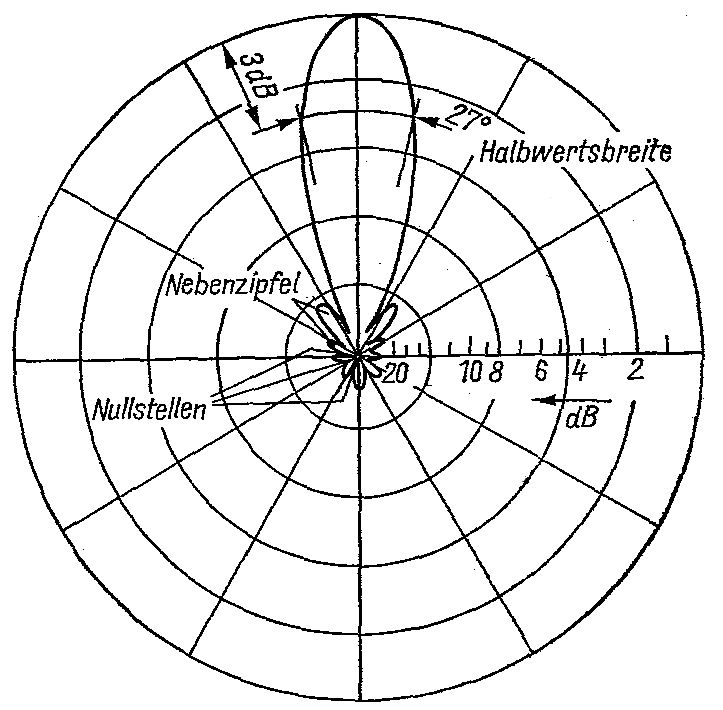
\includegraphics[width=\textwidth]{../ref/Richtdiagramm_Beispiel}
	\caption{Richtdiagramm einer stark bündelnden Antenne}
	\label{fig:Richtdiagramm Beispiel}
\end{figure}

Hierbei ist zu bemerken dass in Abbildung \ref{fig:Richtdiagramm Beispiel} entgegen der üblichen Konvention das Richtdiagramm aus dem Verhältnis zwischen Strahlungsleistungsdichte und ihrem Maximalwert ergibt. Es ist gebräuchlich, das Diagramm auf den Maximalwert zu normieren, sodass sich bei der maximalen Feldstärke 0 dB Dämpfung ergeben.\\
\newline
Der größte Teil der Leistung ist naheliegend in der Hauptkeule zu finden, während es nötig ist die Neben-und Rückwärtskeulen möglichst klein zu halten, um unnötige Abstrahlung in die Umgebung zu vermeiden. Die Halbwertsbreite der Hauptkeule ist der Wert ab dem die Leistungsdichte auf die Hälfte abgesunken ist.\\
\newline
Eine weitere wichtige Kenngröße bei Richtantennen ist das Vor-Rückwärtsverhältnis. Dies ist die Fähigkeit einer Richtantenne, Strahlung aus anderen Richtungen als der Hauptstrahlrichtung zu unterdrücken.

\subsubsection{Einfluss der Erde auf das Richtdiagramm}
Wird das Strahlungsdiagramm einer Antenne über dem Boden mit dem einer Antenne im Freiraum verglichen, lassen sich große Unterschiede erkennen. Der Boden dient als Reflektor wobei seine Reflexionseigenschaften von der Dielektrizitätskonstante sowie der Leitfähigkeit bestimmt werden.\\
\newline
Für die Reflexion elektromagnetischer Wellen am Erdboden trifft das Reflexionsgesetz zu, das bedeutet, dass der Einfallswinkel gleich dem Ausfallswinkel ist. Hierbei kann es zu Überlagerungen zwischen den reflektierten und nicht reflektierten Wellen kommen und somit können destruktive und konstruktive Interferenzen entstehen.\\
\newline
Die Polarisierung der verwendeten Antenne spielt eine entscheidende Rolle bei der Reflexion. Bei einer vertikal polarisierten Antenne ist der Stromverlauf von Spiegelbild und Original gleichphasig. Bei einer horizontal polarisierten Antenne hingegen ist der Stromverlauf zwischen Reflexion und Original gegenphasig.\\
\newline
Der Abstand vom Boden spielt ebenfalls eine kritische Rolle und hat großen Einfluss auf das resultierende Richtdiagramm der Antenne. Wird beispielsweise ein Dipol $\frac{\lambda}{2}$ vom Boden entfernt aufgestellt, so verändert sich sein Richtdiagramm so sehr, dass aus der omnidirektionalen Antenne ein Strahler mit zwei Strahlungskeulen wird. 

\subsection{Antennentypen}
Um ein grundlegendes Verständnis für die in der Diplomarbeit aufgebauten und charakterisierten Antennentypen zu vermitteln, werden diese nun näher erläutert.

\subsubsection{Dipol}

\subsubsection{QFH (Quadrifilar Helical Antenna)}

\subsection{Baluns}

\subsubsection{Strombalun}
Mantelwellensperre, schwach gegen statische Entladungen, da Balun -> konvertiert balanced zu unbalanced 

\subsubsection{Spannungsbalun}
Konvertiert "balanced" zu "unbalanced" guter Schutz gegen statische Entladung, keine Mantelwellensperre.

\subsubsection{Un-Un}